\chapter{Introduction}
\label{chap:SPH}

\section{Abrasive water jet machining}
Material erosion with a high-pressure water jet with abrasives is widely found
in the industry applied to design machining of
metals~\citep{llanto_recent_2021}, composites~ \cite{alberdi_composite_2013}.
Such machining is widely known as abrasive water jet machining (AWJM). AWJM is
used for cutting metallic sheet, glass, and composite materials for automobile,
housing, and aircraft
industries \citep{alberdi_composite_2013,aich_abrasive_2014,llanto_recent_2021},
respectively.
\begin{figure}
  \centering
  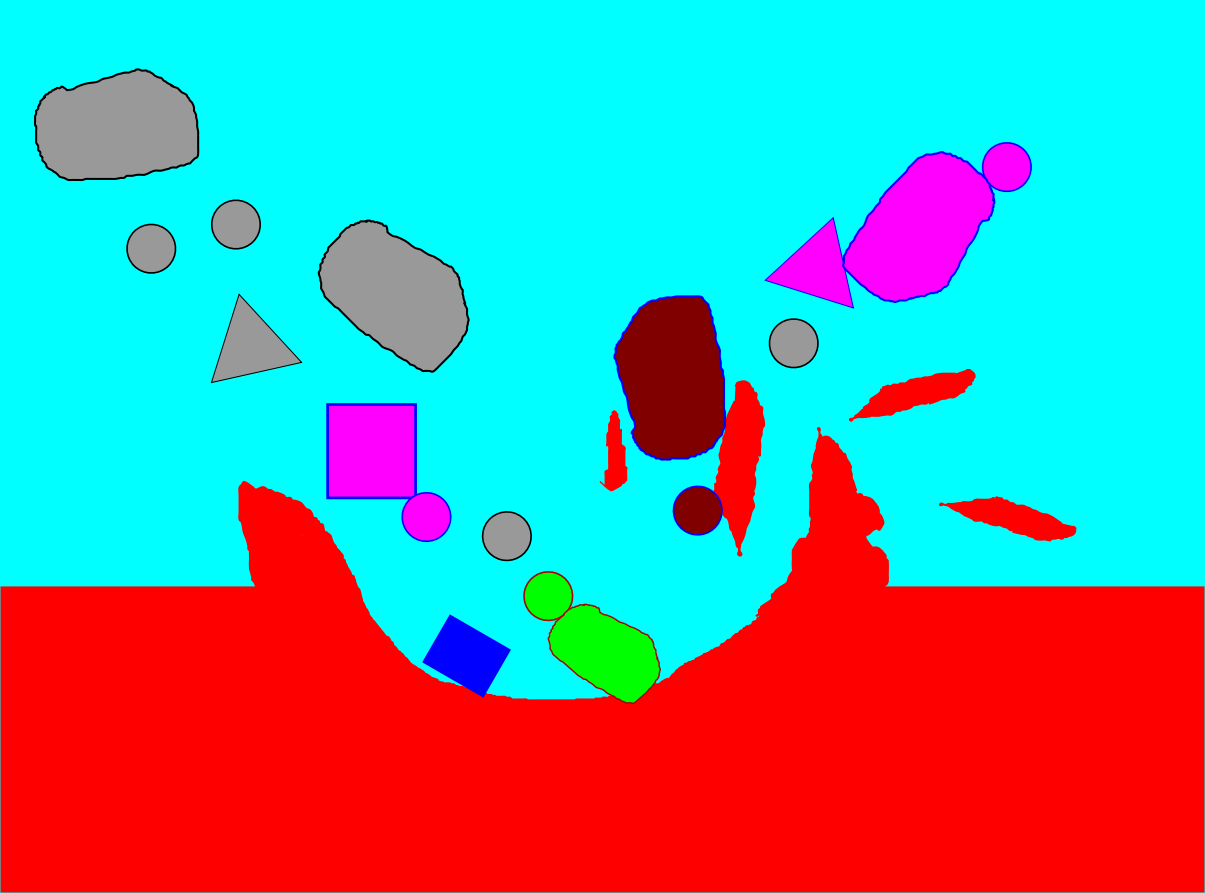
\includegraphics[width=0.5\textwidth]{images/intro/images/intro_section/big_picture}
  \caption{}
\label{fig:intro-big-picture}
\end{figure}
\Cref{fig:intro-big-picture} describes the erosion of brittle solid due to the
impact of rigid bodies in a fluid flow. To model AWJM accurately, we need to
model the incoming fluid dynamics, elastic-plastic behavior of the target, rigid
body dynamics of the impactor, collision handling among the impactors and
between the impactor and the target, two way coupling between the fluid flow and
impactor, and the elastic structure, called as fluid-structure interaction. An
analytical study of AWJM is not possible as it is highly nonlinear and involves
several different multi-physical processes. Therefore, we choose numerical
modeling due to its flexibility in handling nonlinear behavior. Test cases with
exact analytical solutions and experimental cases can be used to develop
numerical techniques while handling each physical process. Mesh-based and
meshless techniques are used to model the AWJM numerically.


% \textbf{Write about SPH and why we choose SPH, about software, updated
%   Lagrangian open source, DEM, runs on all architectures}.


\section{State of the art}

\subsubsection*{Modeling of fluid and elastic dynamics in SPH}

The smoothed particle hydrodynamics (SPH) method has been widely applied since
it was originally proposed to simulate hydrodynamic problems in astrophysics
independently by \citet{lucy77}, and \citet{monaghan-gingold-stars-mnras-77}. It
has been extensively applied to simulate problems involving
fluids~\citep{dalrymple2001sph,shao2003incompressible} in particular to both
compressible~\citep{monaghan-review:2005}, incompressible fluid
flows~\citep{sph:fsf:monaghan-jcp94,sph:psph:cummins-rudman:jcp:1999} as well as
elastic dynamics problems~\citep{randles-1996,gray-ed-2001}, fluid-structure
interaction \citep{khayyer2018enhanced,he2017coupled}, granular physics
\citep{bui2008lagrangian,bui2021smoothed} among other areas.
\cite{monaghan2012smoothed} provides a detailed review of SPH and its
applications.

% in addition to a
% variety of other problems~\citet{rafiee:fsi-2009,khayyer-fsi-2018,
%   sun2021accurate, bui2008lagrangian}.


% The SPH method is a meshless numerical method originally proposed by
% \cite{gingold1977smoothed} and \cite{lucy1977numerical} to model
% astrophysics problems. structural dynamics \citep{randles1996smoothed,dong2016smoothed},



The SPH method is meshless and Lagrangian, and therefore particles move with the
local velocity. This motion can introduce disorder in the particles and thereby
significantly reduce the accuracy of the method. \cite{acc_stab_xu:jcp:2009}
proposed an approach to shift the particles so as to obtain a uniform
distribution of particles. This significantly improves accuracy and the method
is referred to as the Particle Shifting Technique (PST). Many different kinds of
PST methods are available in the
literature~\citep{diff_smoothing_sph:lind:jcp:2012,fickian_smoothing_sph:skillen:cmame:2013,huang_kernel_2019,ye2019sph}.
An alternative approach that ensures particle homogenization for incompressible
fluid flow was proposed as the Transport Velocity Formulation
(TVF)~\citep{Adami2013}. The method introduced an additional stress term to
account for the motion introduced by the particle shifting. The TVF produces
very accurate results but only works for internal flows. \cite{zhang_hu_adams17}
proposed the Generalized Transport Velocity Formulation (GTVF) thereby allowing
the TVF to be used for free-surface problems as well as elastic dynamics
problems. This allows for a unified treatment of both fluids and solids.
Similarly, \cite{oger_ale_sph_2016} introduce ideas from a consistent ALE
formulation for improving the accuracy of SPH. They employ a Riemann-based
formulation to solve fluid mechanics problems and introduce particle shifting to
obtain highly accurate simulations for internal and free-surface problems may
also be handled. The PST has also been employed in the context of the
$\delta$-SPH schemes\citep{sun_consistent_2019}.


The Entropically Damped Artificial Compressibility SPH scheme
(EDAC-SPH)~\citep{edac-sph:cf:2019} introduces an evolution equation for the
pressure and significantly reduces the noise in the pressure since it features
a pressure diffusion term. The approach has a thermodynamic
justification~\citep{Clausen2013} and produces very accurate
results~\citep{edac-sph:cf:2019}.


Recently, \cite{antuono2021delta} carefully combine the ALE-SPH method of
\cite{oger_ale_sph_2016} and the consistent $\delta$-SPH formulation of
\cite{sun_consistent_2019} to improve the accuracy of the $\delta$-SPH
method. They show the importance of the additional terms to the accuracy.


Modeling of elastic solids in SPH was first proposed by
\cite{libersky1991smooth}, where the authors studied the high-speed impact
problems. Despite SPH being applied to elastic solid modeling, it suffers from
tensile instability~\citep{swegle1995smoothed}. The tensile instability problem
has given rise to the total Lagrangian SPH \citep{bonet2002alternative,
  vignjevic2006sph, belytschko2000unified}, where the derivatives of particle
properties are computed in the reference configuration using the deformation
gradient. The updated Lagrangian approach is used by \cite{gray2001sph} and
\cite{monaghan2000sph} where an artificial stress term is introduced to control
instabilities. Many other variants of the updated Lagrangian SPH have been
proposed. Godunov SPH \citep{sugiura2017extension} utilizes a Riemann solver to
reduce the usage of artificial viscosity and a new equation of state is
formulated to solve the tensile instability problem. \cite{dyka1995approach}
uses two sets of particles, where one set of particles stress is computed, and
the other set of particles are used for the evolution of other properties,
through which the tensile instability has been overcome.
\cite{zhang2017generalized} extended the transport velocity formulation (TVF) of
\cite{adami2013transport} to structural dynamics problems and free-surface fluid
mechanics problems. Here the particles are moved with a transport velocity
rather than the momentum velocity to ensure a more homogeneous particle
distribution. This approach also solves the tensile instability problem.


\subsubsection*{Collision SPH}
The dynamics of the projectiles can be modeled by assuming the bodies to be
rigid, as done in the discrete element method (DEM) (\citep{zhan2021surface}).
However, this does not consider any elastic or elastic-plastic deformations of
these colliding bodies. In these cases either finite element methods (FEM)
\citep{rodrigues2019elastic} or meshless methods such as material point
method\citep{sulsky1994particle} or smoothed particle hydrodynamics (SPH)
\citep{gingold1977smoothed} can be used. In this context meshless methods, such
as the SPH method, are advantageous when modeling large deformation of solids as
they do not suffer from issues such as mesh entanglement.

SPH has been successful in modeling the collision between the elastic as well as
elastic-plastic solids \citep{gray2001sph, cleary2010elastoplastic}.
\cite{yan2021simulation} introduced the interfacial SPH scheme, where the SPH
forces are computed only within each body but the interaction between two bodies
is computed using a repulsive force inspired from ABAQUS.
\cite{vyas2021collisional} has modeled the interaction between a rigid body with
an elastic solid, using a penalty-based contact force model.
\cite{mohseni2021particle} use a contact model in order to simulate the
collision between non-smooth rigid bodies with elasto-plastic targets. In both
\citep{vyas2021collisional} and \citep{mohseni2021particle} the friction between
the rigid body and target is considered.


\subsubsection*{Fluid-structure interaction}
The interaction between the ductile target and the incoming jet can be
considered as a fluid-structure interaction phenomenon. Mesh-based schemes such
as finite element method (FEM) \citep{lozovskiy2015unconditionally} and finite
volume method (FVM) \citep{jasak2007updated} have been used for the last few
decades in modeling the FSI problems. However, mesh-based methods are not
favorable when dealing with free surface flow problems or problems involving
large deformation of the structure. This is due to explicit free surface
tracking, and mesh distortion \citep{moresi2003lagrangian} while dealing with
large deformation solids. Therefore, meshless methods are preferred while
handling FSI problems involving free surfaces, multiphase flows, and large
deformation in solids. The smoothed particle hydrodynamics (SPH) and material
point method (MPM) are more commonly used to model the fluid phase. While the
solids are modeled with SPH or Reproducing Kernel Particle Methods (RKPM), or
the Discrete Element Method (DEM) \citep{hu2010material,li2022material}. These
meshless techniques have been coupled for the past two decades to model the
fluid-structure interaction. A few schemes with SPH and MPM are SPH-DEM~
\citep{wu2016coupled}, SPH-TLSPH~\citep{salehizadeh2022coupled},
SPH-RKPM~\citep{peng2021coupling}, SPH-Peridynamics~\citep{sun2020smoothed},
MPM-DEM~\citep{singer2022partitioned}. For more, see the review by
\citep{khayyer2022systematic}.



\subsubsection*{Rigid-fluid coupling and rigid-rigid interaction}
Assuming the incoming projectiles as rigid bodies, the influence of rigid body
on the incoming jet and vice versa is modeled as rigid fluid coupling. In rigid
fluid coupling problems, mesh-based schemes \citep{dettmer_computational_2006}
have been in practice to model fluid dynamics for several decades. However,
these schemes are unfavorable when dealing with free surface flows and mediums
undergoing huge deformation \citep{walkley_finite_2005}. Meshless methods have
been advantageous in modeling free surfaces and large deformations problems.
Therefore, meshless techniques are preferred in addressing these problems. Among
many meshless techniques, moving particle semi-implicit (MPS) - discrete element
method (DEM) \citep{guo2017numerical} and smoothed particle hydrodynamics
(SPH)-DEM \citep{canelas2016sph} are two coupling strategies used to handle
rigid-fluid coupling problems. The rigid body interaction is modeled with DEM.
In addition to DEM, works where SPH \citep{amicarelli2015smoothed} is used to
model the rigid-rigid interaction. However, it lacks to incorporate the friction
between the bodies. MPS and SPH are used to model the fluid phase, and a
coupling strategy is utilized to model the interaction between the rigid body
and the fluid phase.

\cite{cundall_discrete_1979} proposed DEM to study discrete granular materials.
In DEM, the particle dynamics follow simple Newtonian force laws and interact at
their surfaces through a contact force. A shape, mass, and moment of inertia are
assigned to each particle, and originally the particles are assumed to have a
spherical shape. Variations of the DEM were proposed to handle bodies with
different shapes, such as dilated polyhedral DEM \cite{liu_new_2020}, Fourier
series-based discrete element method \cite{lai_fourier_2020}
Gilbert-Johnson-Keerthi(GJK)-DEM \citep{wachs2012grains3d}, discrete function
representation based DEM \citep{lu2012critical}, level set DEM method
\citep{duriez2021precision}. Interaction between bodies with irregular
geometries is modeled by multi-sphere approach \citep{kruggel-emden_study_2008},
surface mesh represented(SMR)-DEM ~\cite{zhan2021surface}.


\subsubsection*{Solid particle erosion}

In theoretical studies, \cite{finnie1972some}, \cite{bitter1963study}
studied the surface erosion of ductile and brittle materials. An analytical
expression for the material removal at different angles of impact is derived in
these studies. Further, an analytical study is carried out by
\cite{hutchings1977erosion}, who provides various results relating the
crater depth, erosion rate related to the impactor particles. In numerical
modeling, mesh based methods are in use for the past few decades in modeling the
solid particle erosion. \cite{molinari2002study,takaffoli2009finite} has
studied the single impact problem using FEM. Meshless techniques are been used
in studying the erosion process, this is due to its advantage in handling
problems with large deformation. \cite{dong2016smoothed} uses smoothed
particle hydrodynamics (SPH) to model the erosion of a ductile target.


\section{Motivation}

\subsubsection*{Numerical modeling of fluid and elastic dynamics in SPH}
SPH in modeling fluid and structural dynamics. Faces several issues and many
different additions were proposed to solve the issues. Transport velocity
formulation is used extensively to solve the particle homogenization problems.
With the notable exception of the GTVF scheme~\citep{zhang_hu_adams17}, most
other applications of the PST have been in the context of fluid mechanics. The
GTVF method provides a unified approach to solve both weakly-compressible fluids
as well as solids. However, the method suffers from a few issues. In order to
work for free-surface problems the method relies on using a different background
pressure for each particle and introduces a few numerical corrections to work
around issues. For example, the smoothing length of the homogenization force is
different from that used by the other equations and this parameter is somewhat
ad-hoc. For solid mechanics problems the method uses the transport velocity of
the particle rather than the true velocity in order to compute the strain and
rotation tensor. In addition there are some terms in the governing equations
that are ignored which play a major role. We also note that the method is not
robust to a change in the particle homogenization force. The EDAC-SPH method
uses the TVF formulation for internal flows and for free-surface flows it does
not employ any form of particle shifting.


\subsubsection*{Elastic solids collision}

Though, SPH~\citep{gray2001sph} has been successful in modeling the collision
between the elastic solids, it does not consider friction between the colliding
solids. Another problem is that the model generates spurious forces on bodies
which are moving close to each other (within the influence radius of the SPH
particles) but not actually interacting. \cite{yan2021simulation} introduced the
interfacial SPH scheme, which eliminates the spurious interactions but it can
not handle friction between the solids. The interaction force does not consider
the shape of the solids in contact. \cite{mohseni2021particle} models the
interaction between a rigid body and a ductile solid using a contact force
model, where the bodies are divided as being primary and a secondary. In
\citep{mohseni2021particle}, the primary body is usually treated as the rigid
body and the body on which the erosion is simulated is treated as secondary.
\cite{vyas2021collisional} also consider the collision between a rigid and
elastic body. \cite{vyas2021collisional} where too there is a clear distinction
between primary and secondary bodies. It is not clear what would happen if both
bodies were elastic or if there is no clear way to distinguish between a primary
and secondary body. \cite{vyas2021collisional,mohseni2021particle} works are not
applied to model the interaction between elastic solids.


\subsubsection*{Fluid-structure interaction and rigid-fluid coupling}
The dynamics of the interaction between ductile target and the incoming jet is
considered as fluid-structure interaction. With meshless techniques preferred in
free surface and large deformation problems. Several different meshless
techniques are coupled in order to simulate the FSI phenomenon. FSI in SPH alone
is modeled by several works, such as, WCSPH-Total Lagrangian SPH (TLSPH)
\citep{zhan2019stabilized}, WCSPH-Updated Lagrangian SPH (ULSPH)
\citep{antoci2007numerical}, ISPH-TLSPH\citep{salehizadeh2022coupled}. However,
using only an updated Lagrangian framework with transport velocity formulation
no work is reported in modeling FSI.

Movement of arbitrarily shaped rigid projectiles are modeled using a
multi-sphere and SMR-DEM approach. However, multi-sphere approach fails to
handle the contact accurately with bodies involving sharp corners, as the force
law assumes the contact between two spherical particles. SMR-DEM requires
additional information to handle the collision, such as connectivity between the
particles comprising the body in addition to the particle positions. However, we
need additional sets of particles to handle the interaction between the rigid
body and the fluid particles. \cite{mohseni2021particle} proposed a new contact
force law, which handles the collision between the bodies based on particle
positions alone. Here the amount of overlap between the bodies is computed using
an SPH method. Utilizing \citep{mohseni2021particle} to model contact between
the bodies allows us to handle the interaction between the fluid particles with
the same set of particles in contrast to SMR-DEM ~\cite{zhan2021surface}.
However, \citep{mohseni2021particle} is applied to contacts involving rigid and
a ductile solids. \citep{mohseni2021particle} is not applied to model the
interaction between inelastic rigid bodies, and in problems involving fluids.


\subsubsection*{Solid particle erosion}
FEM~\citep{takaffoli2009finite} is successful in modeling solid particle
erosion, however, it fails to model the erosion due to many particles. Further,
FEM is not suitable for modeling multiphysics problems, as AWJM has rigid fluid
coupling, FSI in addition to modeling fluid and elastic dynamics.
\cite{dong2016smoothed} uses smoothed particle hydrodynamics (SPH) to model the
erosion of a ductile target. However, \cite{dong2016smoothed} does not consider
the arbitrary shape of the projectile. Further, collision among the projectiles
while interacting with the target is not modeled in SPH. To the authors
knowledge there is no open-source implementation in the literature which can
model the solid particle erosion in SPH.

To develop an open-source framework to model the physics involved in AWJM in SPH.
The following are the key goals of the work.
\begin{itemize}
\item Develop a unified technique in SPH to solve both fluid and solid dynamics
  problems.
\item Handle the collision between the elastic solids using a penalty-based contact force.
\item Develop a fluid-structure interaction solver.
\item Handle the collision among the arbitrarily shaped rigid projectiles in fluid
  flow. Solve the two-way coupling between the fluid and the rigid bodies.
\item Provide an open-source implementation for solid particle erosion in SPH.
\end{itemize}


In this work we propose a scheme which we called Corrected Transport Velocity
Formulation (CTVF) that is inspired by the various recent developments but is
consistent and which works for both solid mechanics and fluid mechanics
problems. We derive the transport velocity equations afresh and note that
there are some important terms that are ignored in earlier approaches using
TVF. These terms are significant and improve the accuracy of the method.
Similar to \cite{oger_ale_sph_2016,sun_consistent_2019}, we detect the free
surface particles and compute their normals using a simpler and
computationally efficient approach which does not require the computation of
eigenvalues. This allows the method to work with free-surfaces without the
introduction of numerical parameters or a variable background pressure. We
employ the EDAC formulation and show that there are additional correction
terms in the EDAC scheme that should be introduced to improve the accuracy of
the method. Furthermore, we show how the EDAC scheme can be used in the
context of solid mechanics problems. We make use of the particle velocity
rather than the transport velocity to compute the velocity gradient, strain,
and rotation rate tensors. Our method can be used with any PST and we consider
the method of \citet{sun_consistent_2019} as well as the iterative PST of
\citet{huang_kernel_2019}. The method is also robust to the choice of the
smoothing kernel. The resulting method works for both weakly-compressible
fluids as well as solids. The new method may be thought of as an improved
extension of the EDAC-SPH method that can be used for free-surface problems as
well as solid mechanics problems.


In the current work, the collision between elastic solids is modeled using a
penalty-based contact force model. Unlike the approach of
\cite{yan2021simulation}, the proposed contact force model can handle friction
between the solids as well. The bodies themselves are elastic and this is
simulated using the CTVF SPH method \cite{adepu2021corrected}. The penalty-based
force considered here is the one proposed by \citet{mohseni2021particle}. In the
original model proposed by \cite{mohseni2021particle}, the contact force is
between a primary body and a secondary body. In \cite{mohseni2021particle}, the
primary body is usually treated as the rigid body and the body on which the
erosion is simulated is treated as secondary. It is not clear what would happen
if both bodies were elastic or if there is no clear way to distinguish between a
primary and secondary body. We explore the importance of choosing the primary
and secondary body under collision.

In the current work, we handle FSI problems by the CTVF method, where both
fluids and solid phases are modeled using CTVF alone. We couple CTVF with DEM to
model the rigid fluid coupling problems. The fluid phase is handled using a
corrected transport velocity formulation developed by \cite{adepu2021corrected},
which provides smooth pressure distribution with EDAC formulation and
homogeneous particle distribution, resulting in accurate fluid modeling. While
DEM is used to handle rigid-rigid interactions and applied to 3D problems, and
it is further modified to handle inelastic collisions by introducing a damping
term in the contact force equation. The interaction between the fluid phase and
rigid bodies is handled using the dummy particle approach \citep{Adami2012}.


\section{Overview}
The current thesis is organized in the following way. The current chapter
introduces the basic formalism of SPH. In the next chapter, \cref{chap:ctvf}, we
introduce corrected transport velocity formulation in SPH and apply it to model
the dynamics of fluids and elastic structures. The new formulation eliminates
several issues SPH faces. \Cref{chap:csph} improvises the collision model by
incorporating a contact force model in SPH while the bodies are colliding. This
essentially eliminates spurious interaction between the bodies and incorporates
friction between the interacting bodies. \Cref{chap:fsi} is utilized to model
the interaction between the elastic structure and the incoming jet. This is
modeled with coupling the solver developed in \cref{chap:ctvf}, here both fluid
and solid phases and coupled using a dummy particle approach. In
\cref{chap:rfc}, we study the dynamics of the projectiles onto the target in an
incoming high-speed jet. We couple CTVF with DEM to model the rigid fluid
coupling phenomenon. The interaction between the rigid bodies is handled with
DEM. \Cref{chap:erosion} models the solid particle erosion of the ductile body
due to an impact of the projectile. The contact force implemented in
\cref{chap:csph} is used to handle the interaction between the rigid body and
the ductile solid. Johnson-Cook constitutive model is utilized to model the
plasticity of the target.


In the next section we introduce the SPH methodology and show how a function,
derivative and divergence operators are approximated.
% We show how SPH is used to
% solve the fluid and elastic solid problems in updated Lagrangian formalism.
% Several issues of SPH is discussed, tensile instability, particle
% inhomogenization, through numerical examples.

\section{Smoothed particle hydrodynamics}
In the current section, we introduce the basics of smoothed particle
hydrodynamics. A fundamental overview of the discrete approximations of
function, derivative, and divergence is discussed. Advanced approximations are
derived, keeping the conservation of quantities in mind.
\subsection{Function approximation}
The function value of a smooth function $A$ defined over a domain $\Omega$ at
point $x$ can be written as
\begin{equation}
  \label{eq:dirac_repr}
  A(\ten{x}) = \int_{\Omega}\> A(\ten{x}') \> \delta(\ten{x} - \ten{x}') \> d\ten{x}'^{n},
\end{equation}
where $\delta(\ten{x} - \ten{x}')$ is a Dirac-delta function having the
following properties,
\begin{equation}
  \label{eq:dirac-delta}
  \delta(\ten{x}) =
  \begin{cases}
    +\infty, & \ten{x} = \ten{0}\\
    0, & \ten{x} \neq \ten{0}
  \end{cases}
\end{equation}
and
\begin{equation}
  \label{eq:unity}
  \int_{\Omega}\> \delta(\ten{x}) \> d\ten{x} = 1.
\end{equation}
Here, $m$ chosen depending on the dimension of the space, $2$ and $3$ for 2D and 3D space.
The exact function value at $x$ can be retrieved by the following steps,
\begin{align*}
  \label{eq:dirac_derivation}
  A(\ten{x}) &= \int_{\Omega}\> A(\ten{x}') \> \delta(\ten{x} - \ten{x}') \> d\ten{x}'\\
  A(\ten{x}) &= A(\ten{x}) \int_{\Omega}\> \> \delta(\ten{x} - \ten{x}') \> d\ten{x}'\\
  A(\ten{x}) &= A(\ten{x})
\end{align*}
In SPH, the Dirac delta function is replaced with a compact smooth function $W$,
chosen to be as even function. The function value of $A$ at $\ten{x}$
interpolated with the smooth kernel $W$ is given by
\begin{equation}
  \label{eq:kernel_repr}
  A(\ten{x}) = \int_{\Omega}\> A(\ten{x}') \> W(\ten{x} - \ten{x}', h)  \> d\ten{x}' + O(h^2).
\end{equation}
Here, kernel $W$ satisfies the unity condition, given by
\begin{equation}
  \label{eq:unity}
  \int_{\Omega}\> W(\ten{x} - \ten{x}', h)  \> d\ten{x}' = 1.
\end{equation}

\begin{equation}
  \label{eq:kernel_delta}
  \lim_{h \to 0} W(\boldsymbol{x} - \boldsymbol{x}', h) = \delta(\boldsymbol{x} - \boldsymbol{x}', h)
\end{equation}
\begin{equation}
  \label{eq:compact_support}
  W(\boldsymbol{x} - \boldsymbol{x}', h) = 0 \>\>\>\>    \text{when}  \>\>\> |\boldsymbol{x} - \boldsymbol{x}'| > kh
\end{equation}
In the current work we have used Quintic spline in all our simulation cases. Quintic spline is given as,
\begin{equation}
  \label{eq:quintic_spline}
  W(r, h) =
  \begin{cases}
    \sigma_5\left( (3-q)^5 - 6(2-q)^5 + 15(1-q)^5 \right), & \textrm{for} \ 0\leq q \leq 1,\\
    \sigma_5\left( (3-q)^5 - 6(2-q)^5 \right), & \textrm{for} \ 1 <  q \leq 2,\\
    \sigma_5 \ (3-q)^5 , & \textrm{for} \ 2 < q \leq 3,\\
    0, & \textrm{for} \ q>3,
  \end{cases}
\end{equation}


This type of interpolation leads to a 2nd order function accuracy (cite
references). Much better kernels can be used to approximate the function, but
that may result in negative density which we want to avoid.

Assume that the domain is discretized into N particles with mass $m_i$ and volume
$dv_i$. We have
\begin{equation}
  \label{eq:mass_repr}
  m_j = dv_i \> \rho_i
\end{equation}

Using \eqref{eq:mass_repr}, \eqref{eq:kernel_repr} is converted to
discrete form as follows

\begin{equation}
  \label{eq:discrete_form}
  A_i = \sum\> \frac{m_j}{\rho_j} A_j\> W(\ten{x}_i - \ten{x}_j, h)
\end{equation}

Where $A_i$ is the value of the field property of particle i,
similarly for $A_j$.

\subsection{Derivative approximation}
Similarly, the continuous SPH interpolation of the derivative of a field variable
is written as
\begin{equation}
  \label{intro:eq:sph-continu-derivative-interpolation}
  \nabla A(\ten{x}) = \int_{\Omega}\> \nabla A(\ten{x}') \> W(\ten{x} - \ten{x}', h)  \> d\ten{x}'^{m}
\end{equation}
By applying integration by parts to the right hand side results in,
\begin{equation}
  \label{eq:sph-continu-derivative-interpolation}
  \nabla A(\ten{x}) = - \int_{\Omega}\> A(\ten{x}') \> \nabla_{\ten{x}'} W(\ten{x} - \ten{x}', h)  \> d\ten{x}'^{m} +
  - \int_{\Omega}\> \nabla \left( A(\ten{x}') \> W(\ten{x} - \ten{x}', h)\right)  \> d\ten{x}'^{m}
\end{equation}
From symmetric property of the kernel $W$, we get the derivative of the kernel
as antisymmetric and thus
\begin{equation}
  \label{intro:eq:sph-kernel-antisymmetric}
  \nabla_{\ten{x}'} W(\ten{x} - \ten{x}', h) = -\nabla_{\ten{x}} W(\ten{x} - \ten{x}', h)
\end{equation}
Furthermore, using the Stokes theorem, the last term of
\cref{eq:sph-continu-derivative-interpolation} can be written as a surface
integral, the resulting equation is
\begin{equation}
  \label{intro:eq:sph-continu-derivative-stokes}
  \nabla A(\ten{x}) = \int_{\Omega}\> A(\ten{x}') \> \nabla_{\ten{x}} W(\ten{x} - \ten{x}', h)  \> d\ten{x}'^{m} +
  - \int_{\partial \Omega}\> \left( A(\ten{x}') \> W(\ten{x} - \ten{x}', h)\right) \ten{n}_{\ten{x}'} \> d\teng{\Gamma}(\ten{x}')
\end{equation}
With the domain being unbounded, and with the compact support property of the
kernel, the above integral becomes,
\begin{equation}
  \label{intro:eq:sph-continu-derivative-final}
  \nabla A(\ten{x}) = \int_{\Omega}\> A(\ten{x}') \> \nabla_{\ten{x}} W(\ten{x} - \ten{x}', h)  \> d\ten{x}'^{m}.
\end{equation}
The discretized form of the above integral derivative approximation is
\begin{equation}
  \label{intro:eq:derivative-discrete_form}
  \nabla A(\ten{x}_i) = \sum\> \frac{m_j}{\rho_j} A_j\> \nabla W(\ten{x}_i - \ten{x}_j, h).
\end{equation}

An alternative expression of the derivative approximation is derived by employing
density, i.e,
\begin{equation}
  \label{intro:eq:sph-continu-derivative-final}
  \nabla (A \rho^n) = n A \rho^{n - 1} \nabla \rho + \rho^n \nabla A,
\end{equation}
where $n$ is a real number. The new identity for the derivative of $A$ is
\begin{equation}
  \nabla A = \frac{1}{\rho^n} \left[ n A \rho^{n - 1} \nabla \rho + \rho^n \nabla A  \right],
\end{equation}
using \cref{eq:discrete_form,intro:eq:derivative-discrete_form}, the new
derivative approximation can be written as
\begin{equation}
  \label{intro:eq:derivative-discrete_form}
  \nabla A(\ten{x}_i) = \frac{1}{\rho^n(\ten{x}_i)} \sum\>
  m_j \left(A_j \rho^{n-1}(\ten{x}_j) - n A_i \rho^{n-1}(\ten{x}_i) \right)\> \nabla W(\ten{x}_i - \ten{x}_j, h).
\end{equation}
In the current work, we use a symmetric expression, we substitute $n=-1$, resulting in
\begin{equation}
  \nabla A(\ten{x}_i) = \rho_i \sum_{j} m_j \left(\frac{A_i}{\rho_i^2} + \frac{A_j}{\rho_j^2}\right) \nabla W_{ij}.
\end{equation}



\subsection{Divergence approximation}
\begin{equation}
  \label{intro:eq:discrete_derivative}
  \nabla \cdot \ten{v}_i = \sum\> \frac{m_j}{\rho_j} \ten{v}_j \cdot \nabla W(\ten{x}_i - \ten{x}_j, h)
\end{equation}
Similar to derivative approximation, we utilize the following calculus identity to,
\begin{equation}
  \label{intro:eq:sph-continu-div-intermediate}
  \nabla \cdot (\ten{v} \rho^n) = \rho^n \nabla \cdot \ten{v} + n  \rho^{n - 1} \ten{v} \cdot \nabla \rho.
\end{equation}
A discrete SPH approximation for $n=1$ is given by,
\begin{equation}
  \label{intro:eq:sph-continu-div-final}
  \nabla \cdot (\ten{v} \rho^n) = \rho^n \nabla \cdot \ten{v} + n  \rho^{n - 1} \ten{v} \cdot \nabla \rho.
\end{equation}



% \section{SPH discretization of the governing equations}

% \subsection{Continuity equation}
% % The continuity equation from chapter 2 \eqref{c02:cont_eqn} is discretized here.
% We employ density based approximation to the divergence, as a golden rule of SPH,
% \begin{equation}
%   \nabla \cdot \ten{A} = \frac{\nabla \cdot (\rho\ten{A}) - \ten{A} \cdot \nabla \rho}{\rho}
% \end{equation}

% \begin{equation}
%   \rho_a \left(\nabla \cdot \ten{A} \right)_a = \sum_b\> \frac{m_j}{\rho_j}
%   \left(\ten{A}_b - \ten{A}_a\right) \cdot \nabla W(\ten{x}_i - \ten{x}_j, h)
% \end{equation}

% \begin{equation}
%   \label{intro:eq:sph-discretization-continuity}
%   \frac{d\rho_a}{dt} = \sum_{b} \; \frac{m_b}{\rho_{b}} \;
%   \rho_{a} \; \ten{u}_{ab} \; \cdot \nabla_{a} W_{ab}
% \end{equation}

% %
% \subsection{Momentum equation}
% An improved approxiation of the gradient is utilized to discretize the momentum
% equation. The new improved gradient can be writen as,
% \begin{equation}
%   \frac{\nabla p}{\rho} = \nabla \left(\frac{\nalba p}{\rho}\right) +
%   \frac{p}{\rho^2} \nabla \rho
% \end{equation}


% For fluid case
% \begin{multline}
%   \label{intro:eq:sph-momentum-fluid}
%   \frac{d\ten{u}_{a}}{dt} = - \sum_{b} m_b
%   \left(\frac{p_a}{\rho_a^2} + \frac{p_b}{\rho_b^2}\right) \nabla_{a} W_{ab}
%   + \sum_{b} m_b \frac{4 \eta \nabla W_{ab}\cdot
%     \ten{r}_{ab}}{(\rho_a + \rho_b) (r_{ab}^2 + 0.01 h_{ab}^2)} \ten{u}_{ab} +
%   \ten{g}_{a},
% \end{multline}


% For solid case
% \begin{equation}
%   \label{intro:eq:sph-momentum-solid}
%   \frac{\tilde{d}\ten{u}_{a}}{dt} = - \sum_{b} m_b \bigg[
%   \bigg(\frac{p_a}{\rho_a^2} + \frac{p_b}{\rho_b^2}\bigg) \ten{I} -
%   \bigg(\frac{\teng{\sigma}^{'}_{a}}{\rho_a^2} +
%   \frac{\teng{\sigma}^{'}_{b}}{\rho_b^2} + \Pi_{ab} \ten{I} \bigg) \bigg]  \cdot \nabla_{a} W_{ab} +
%   \ten{g}_{a},
% \end{equation}

% We add to the momentum equation an additional artificial viscosity term
% $\Pi_{ab}$~\cite{monaghan-review:2005} to maintain the stability of the
% numerical scheme, given as,
% \begin{align}
%   \label{intro:eq:mom-av}
%   \Pi_{ab} =
%   \begin{cases}
% \frac{-\alpha h_{ab} \bar{c}_{ab} \phi_{ab}}{\bar{\rho}_{ab}}
%   & \ten{u}_{ab}\cdot \ten{r}_{ab} < 0, \\
%   0 & \ten{u}_{ab}\cdot \ten{r}_{ab} \ge 0,
% \end{cases}
% \end{align}
% where,
% %
% \begin{equation}
%   \label{intro:eq:av-phiij}
%   \phi_{ab} = \frac{\ten{u}_{ab} \cdot \ten{r}_{ab}}{r^2_{ab} + 0.01 h^2_{ab}},
% \end{equation}
% %
% where $\ten{r}_{ab} = \ten{r}_a - \ten{r}_b$, $\ten{u}_{ab} = \ten{u}_a -
% \ten{u}_b$, $h_{ab} = (h_a + h_b)/2$, $\bar{\rho}_{ab} = (\rho_a + \rho_b)/2$,
% $\bar{c}_{ab} = (c_a + c_b) / 2$, and $\alpha$ is the artificial
% viscosity parameter.


% \begin{equation}
%   \label{intro:eq:sph-vel-grad}
%   \nabla \ten{u}_a =
%   - \sum_{b} \frac{m_b}{\rho_{b}} (\ten{u}_{a} - \ten{u}_{b}) \otimes (\nabla_{a} W_{ab}),
% \end{equation}
% where $\otimes$ is the outer product.

% The SPH discretization of the modified Jaumann stress rate
% \cref{eq:modified-jaumann-stress-rate} is given as,
% \begin{equation}
%   \label{intro:eq:sph-modified-jaumann-stress}
%   \frac{d\teng{\sigma}^{'}_{a}}{dt} = 2G (\dot{\teng{\epsilon}}_{a} -
%   \frac{1}{3} \dot{\teng{\epsilon}}_{a} \ten{I}) + \teng{\sigma}^{'}_{a}
%   \teng{\Omega}_{a}^{T} +
%   \teng{\Omega}_{a} \teng{\sigma}^{'}_{a}
% \end{equation}

% \section{Results}
% The developed technique for modeling the fluid and elastic dynamics is applied
% to a periodic Tarylor-Green vortex problem and to a colliding elastic rings.
% Where we test the fidelity of the basic solver.
% \subsection{Taylor-Green vortex}
% Taylor-Green vortex is a periodic unit box with no solid boundaries. It has an
% exact solution given as,
% \begin{align}
%   \label{intro:eq:tgv_sol}
%   u &= - U e^{bt} \cos(2 \pi x) \sin(2 \pi y) \\
%   v &=   U e^{bt}\sin(2 \pi x) \cos(2 \pi y) \\
%   p &=  -U^2 e^{2bt} (\cos(4 \pi x) + \cos(4 \pi y))/4,
% \end{align}
% where $U$ is chosen as $1$ m\,s\textsuperscript{-1}, $b=-8\pi^2/Re$,
% $Re=U L /\nu$, and $L=1$ m. We initialize the fluid with the above values at
% time $t=0$ and compare the results with the exact solution. The Reynolds number,
% $Re$, is chosen to be $100$. The quintic spline with $h/\Delta x = 1.0$ is used.
% No artificial viscosity is used for this problem.

% \begin{figure}[!htpb]
%   \centering
%   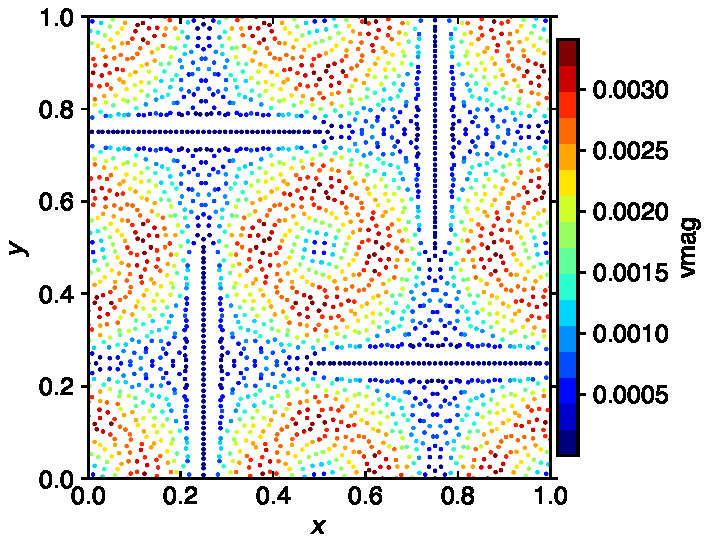
\includegraphics[width=0.5\textwidth]{figures/intro/figures/taylor_green/particle_plot_velocity}
%   \caption{Bodies under collision which are divided into primary and
%     secondary.}
% \label{fig:bodies_under_collision}
% \end{figure}

% \begin{figure}[!htpb]
%   \centering
%   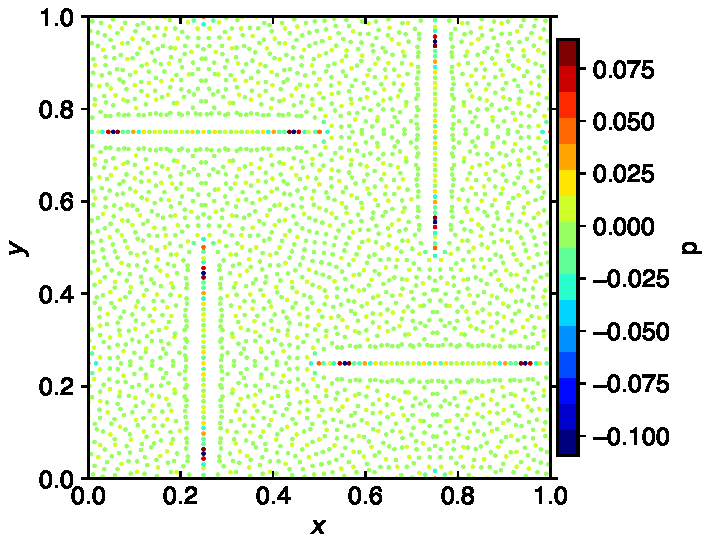
\includegraphics[width=0.5\textwidth]{figures/intro/figures/taylor_green/particle_plot_pressure}
%   \caption{Bodies under collision which are divided into primary and
%     secondary.}
% \label{fig:bodies_under_collision}
% \end{figure}
% % %
% % %
% % The decay rate of the velocity is studied using the evolution of maximum
% % velocity $|\ten{u}_{\max}|$ in time. We compute the $L_1$ error in the
% % velocity magnitude as,
% % \begin{equation}
% %   \label{intro:eq:tg:l1}
% %   L_1 = \frac{\sum_i |\ten{u}_{i, computed}| - |\ten{u}_{i, exact}|}
% %   {\sum_i |\ten{u}_{i, exact}|},
% % \end{equation}
% % where $\ten{u}_{i, exact}$ is found at the position of the $i$'th particle.


% \FloatBarrier%
% \subsection{Colliding Rings}
% \label{colliding-rings}

% We apply the current SPH discretized equations
% Having shown the flexibility of proposed scheme to work with different PST
% methods in \cref{sec:oscillating-plate}, in the current example, we compare
% the robustness of the PST methods by investigating the collision of rubber
% rings with different Poisson ratios. This was first studied in SPH by
% \citet{swegle1995smoothed}.

% The inner ring radius of the ring is $r_{min} = 0.03$ m and the outer ring
% radius $r_{max} = 0.04$ m. Both the rings have the same material properties:
% Young's modulus $E = 0.01$ GPa and density $\rho = 1.2 \times 10^{3}$
%  kg\,m\textsuperscript{-3}. The initial speed of the rings are equal to
% $v_0 = 0.12 c_0$ m\,s\textsuperscript{-1} with an initial inter particle spacing of
% $\Delta x = 0.001$ m. Where $c_0$ is the speed of sound of the material. We use
% an $\alpha=1$ for the artificial viscosity in the current simulation.
% \begin{figure}[!htpb]
%   \centering
%   
\includegraphics[width=0.5\textwidth]{images/intro/images/rings/rings}
%   \caption{Bodies under collision which are divided into primary and
%     secondary.}
% \label{fig:bodies_under_collision}
% \end{figure}

% Two different Poisson ratios are simulated. \Cref{fig:rings:sun2019-nu-0.3975}
% shows the particle positions of rings with a Poisson ratio of $0.3975$ when
% simulated with SPST. The recovery of the colliding rings without any tensile
% instability can be seen.

% We also consider higher Poisson ratios, such as 0.47.
% \Cref{fig:rings:sun2019-nu-0-47} shows the particle positions of rings when
% simulated with SPST and \cref{fig:rings:ipst-nu-0-47} with IPST. Even though
% both the particle shifting techniques are able to eliminate the numerical
% fracture, IPST gives better results as in the distribution of particles
% through out the simulation, see \cref{fig:rings:sun2019-nu-0.47-2} and
% \cref{fig:rings:ipst-nu-0.47-2}. For the case where SPST is used, the final
% particle distribution is not very uniform. This is not the case when IPST is
% used. We can therefore say that IPST performs better than SPST.
% %
% \begin{figure}
%   \centering
%   \begin{subfigure}{0.48\textwidth}
%     \centering
%     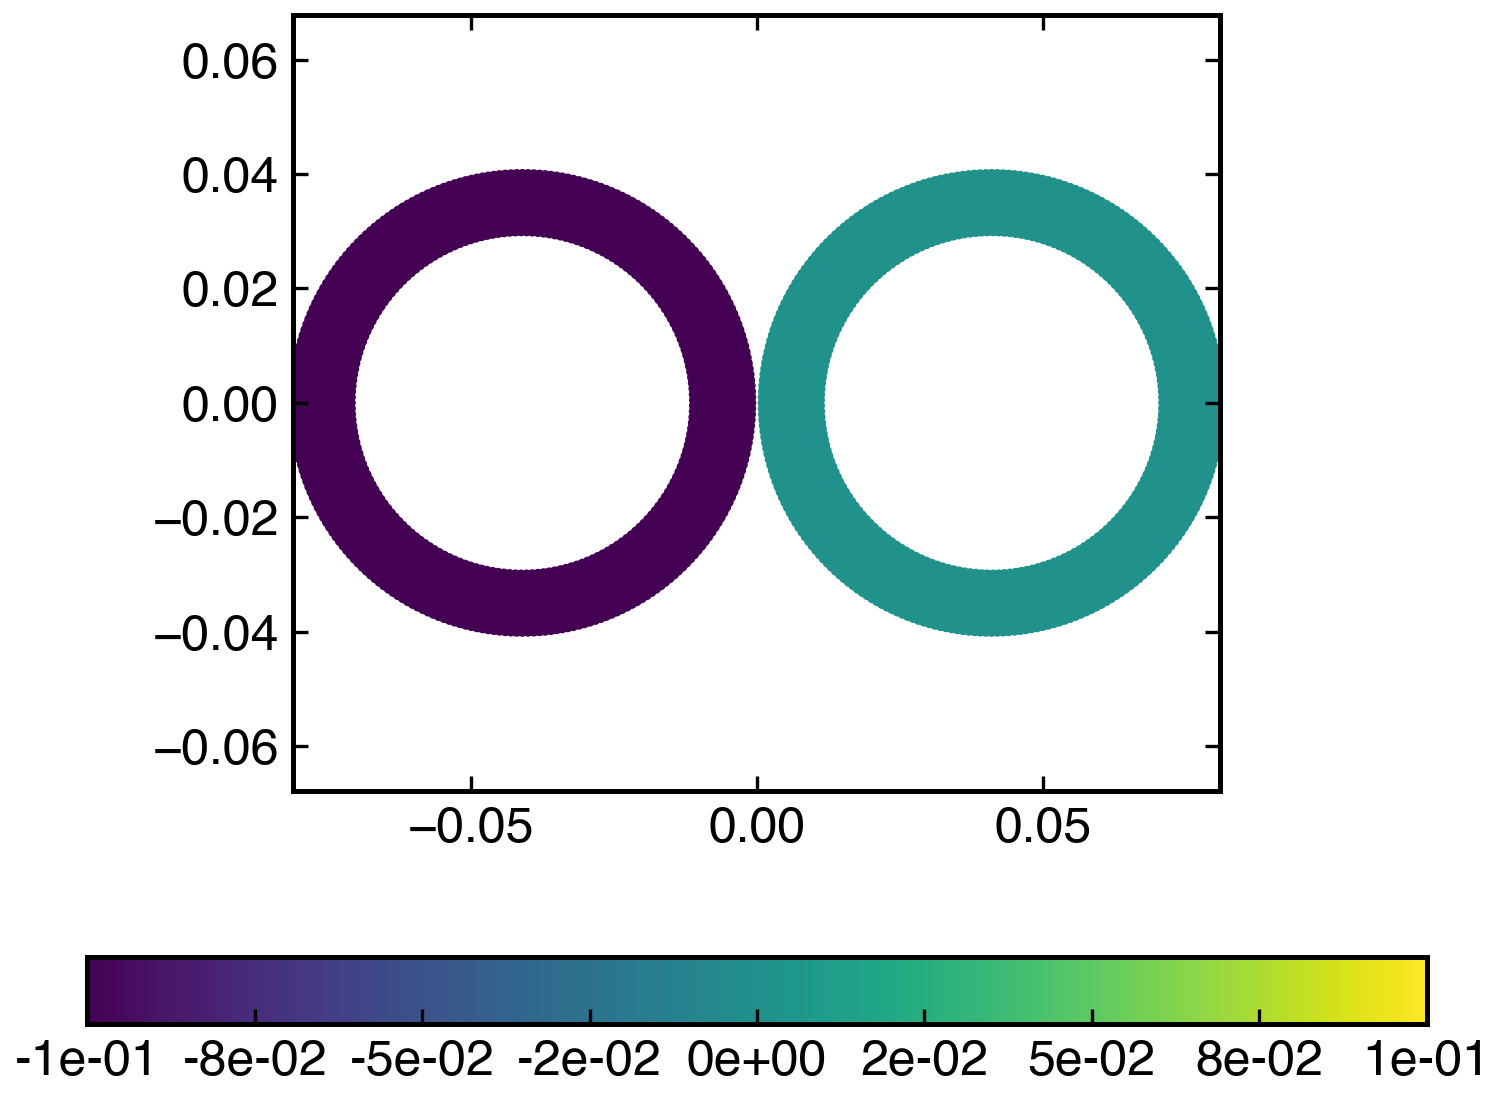
\includegraphics[width=1.0\textwidth]{figures/intro/figures/rings/time0}
%     \subcaption{t = 0 sec}\label{fig:rings:sun2019-nu-0.3975-0}
%   \end{subfigure}
%   %
%   \begin{subfigure}{0.48\textwidth}
%     \centering
%     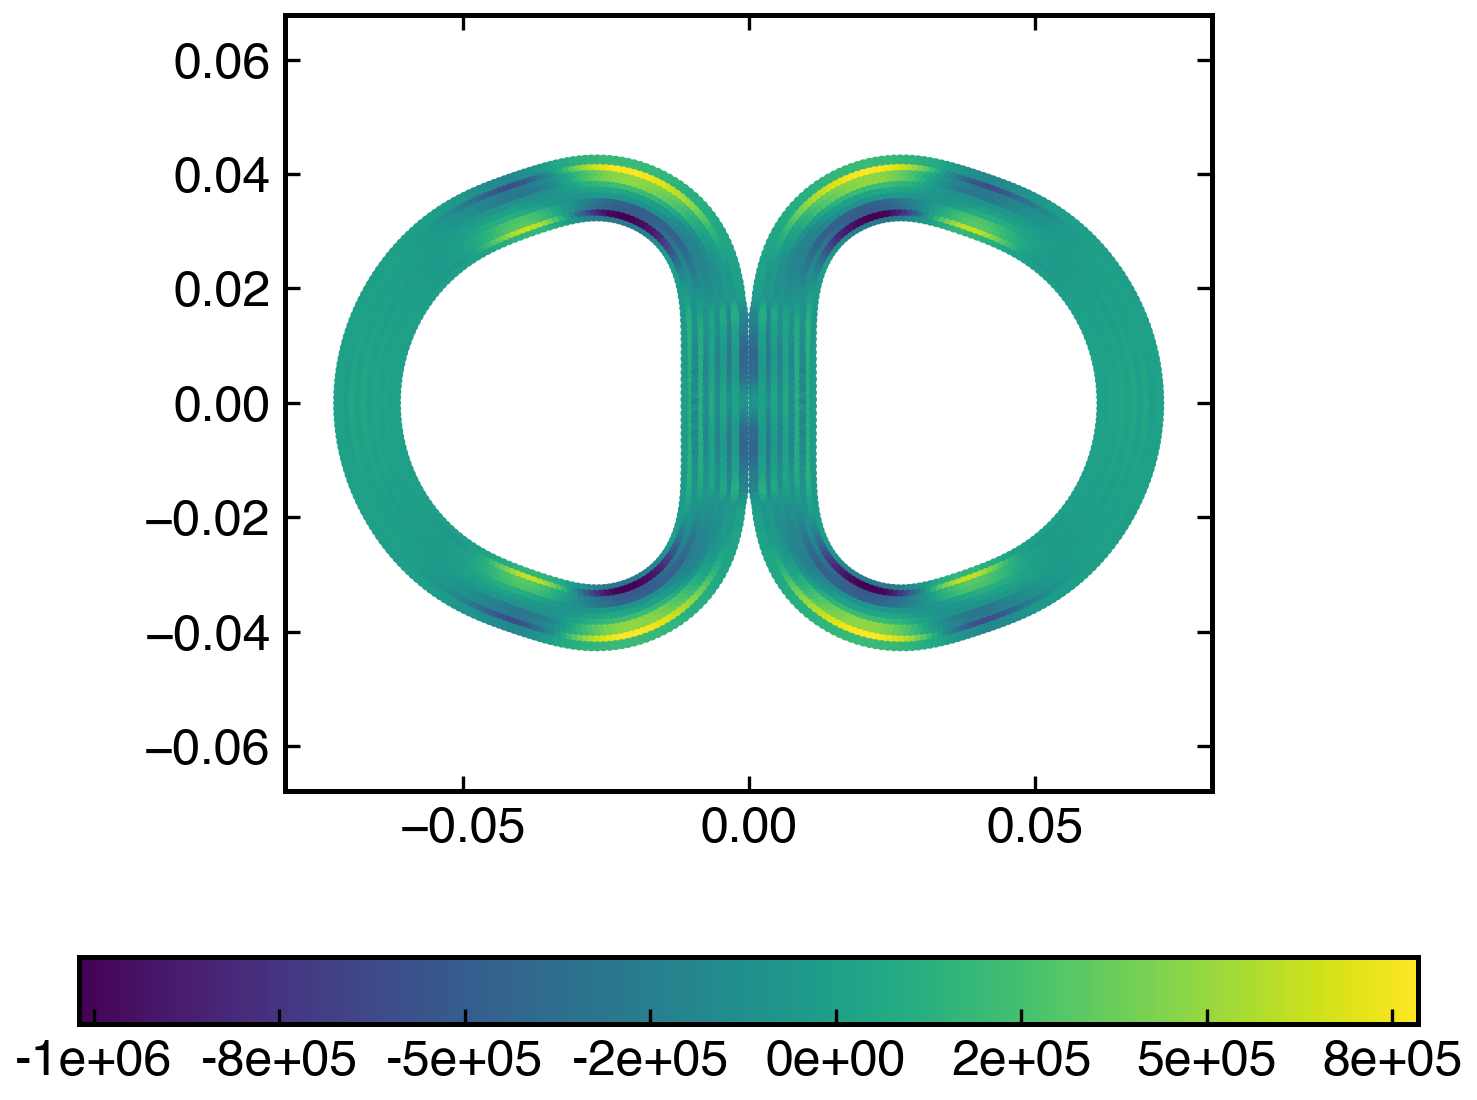
\includegraphics[width=1.0\textwidth]{figures/intro/figures/rings/time1}
%     \subcaption{t = 2.5e-03 sec}\label{fig:rings:sun2019-nu-0.3975-1}
%   \end{subfigure}
% % %
% %   \begin{subfigure}{0.48\textwidth}
% %     \centering
% %     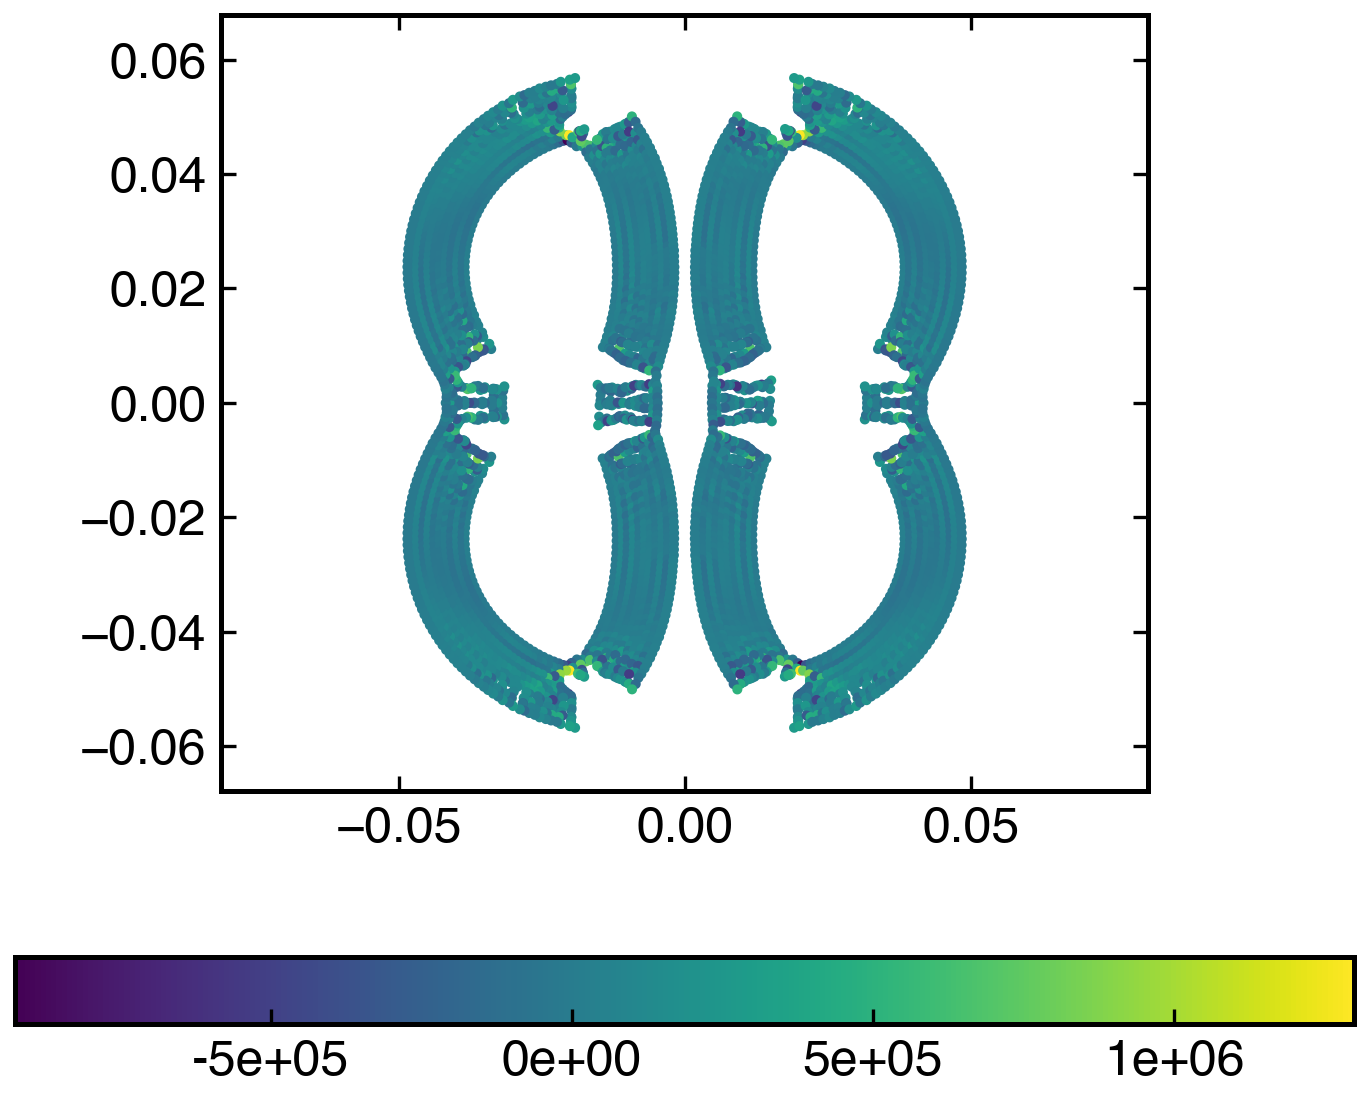
\includegraphics[width=1.0\textwidth]{figures/intro/figures/rings/time2}
% %     \subcaption{t = 4e-03 sec}\label{fig:rings:sun2019-nu-0.3975-2}
% %   \end{subfigure}

%   \begin{subfigure}{0.48\textwidth}
%     \centering
%     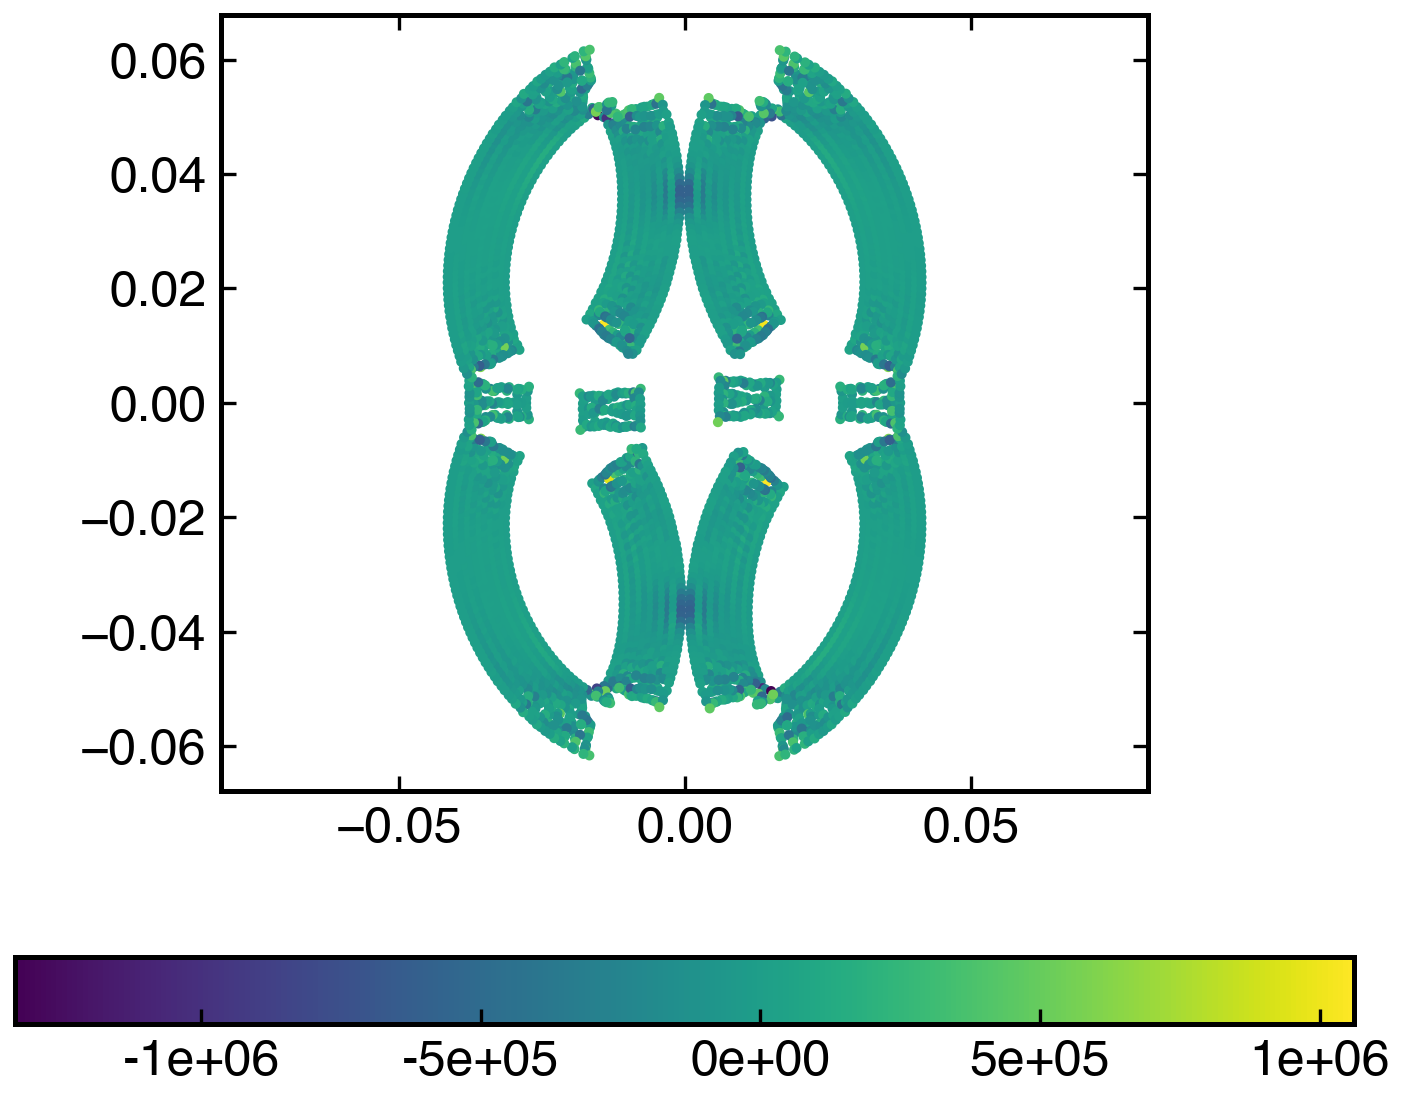
\includegraphics[width=1.0\textwidth]{figures/intro/figures/rings/time3}
%     \subcaption{t = 7.3e-03 sec}\label{fig:rings:sun2019-nu-0.3975-3}
%   \end{subfigure}
% %
%   \begin{subfigure}{0.48\textwidth}
%     \centering
%     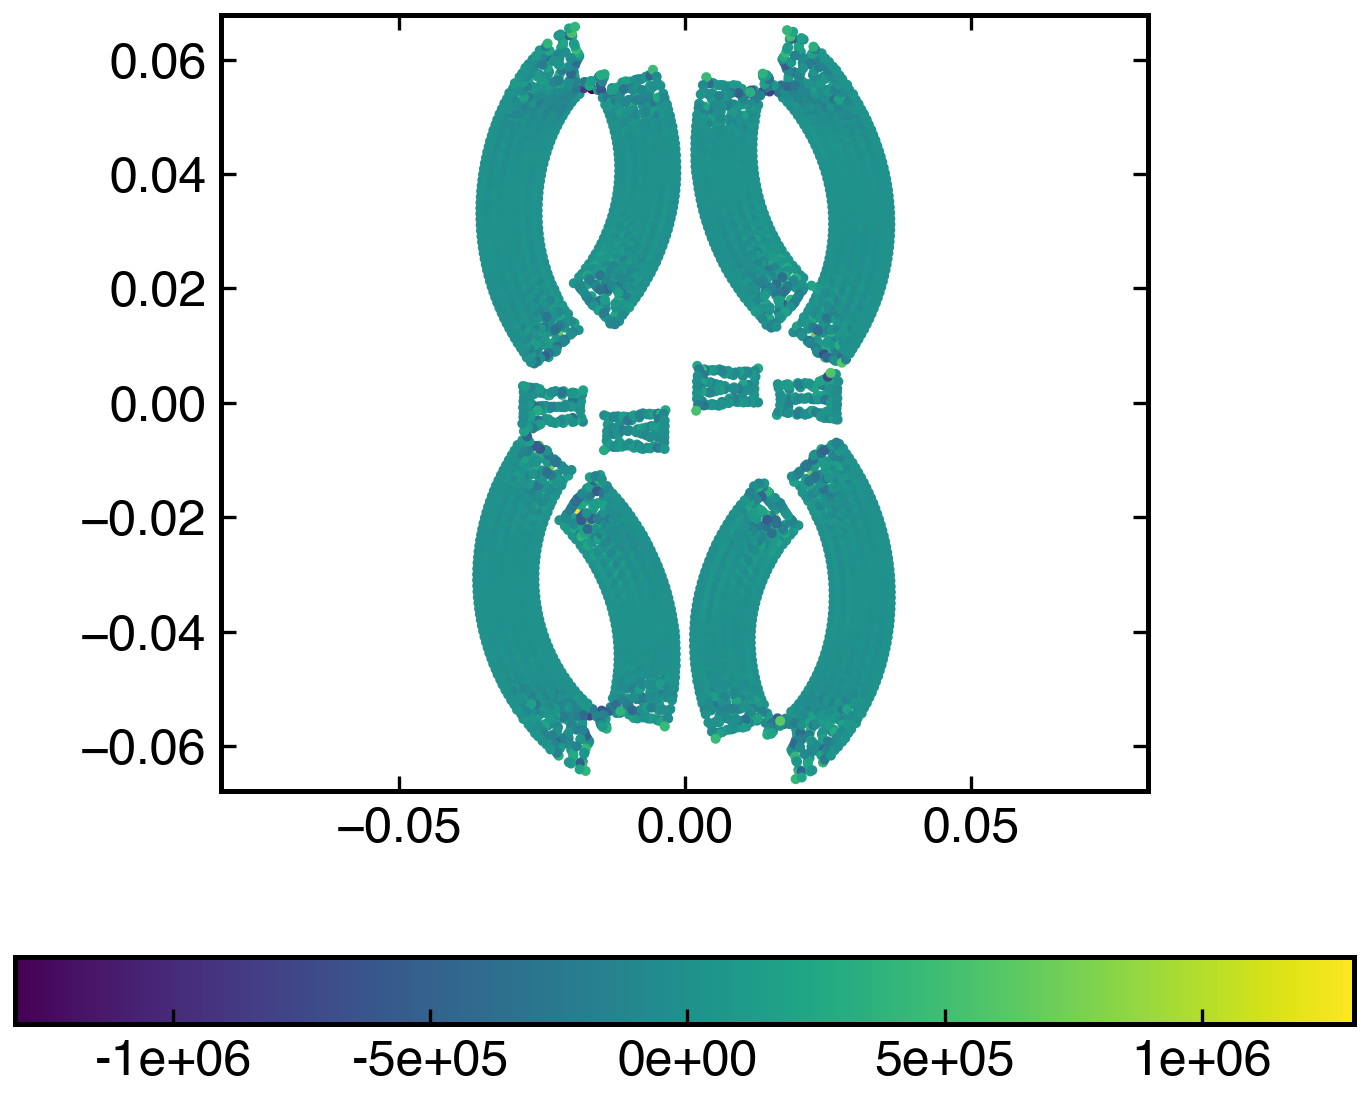
\includegraphics[width=1.0\textwidth]{figures/intro/figures/rings/time4}
%     \subcaption{t = 1.45e-02 sec}\label{fig:rings:sun2019-nu-0.3975-4}
%   \end{subfigure}
% % %
% %   \begin{subfigure}{0.3\textwidth}
% %     \centering
% %     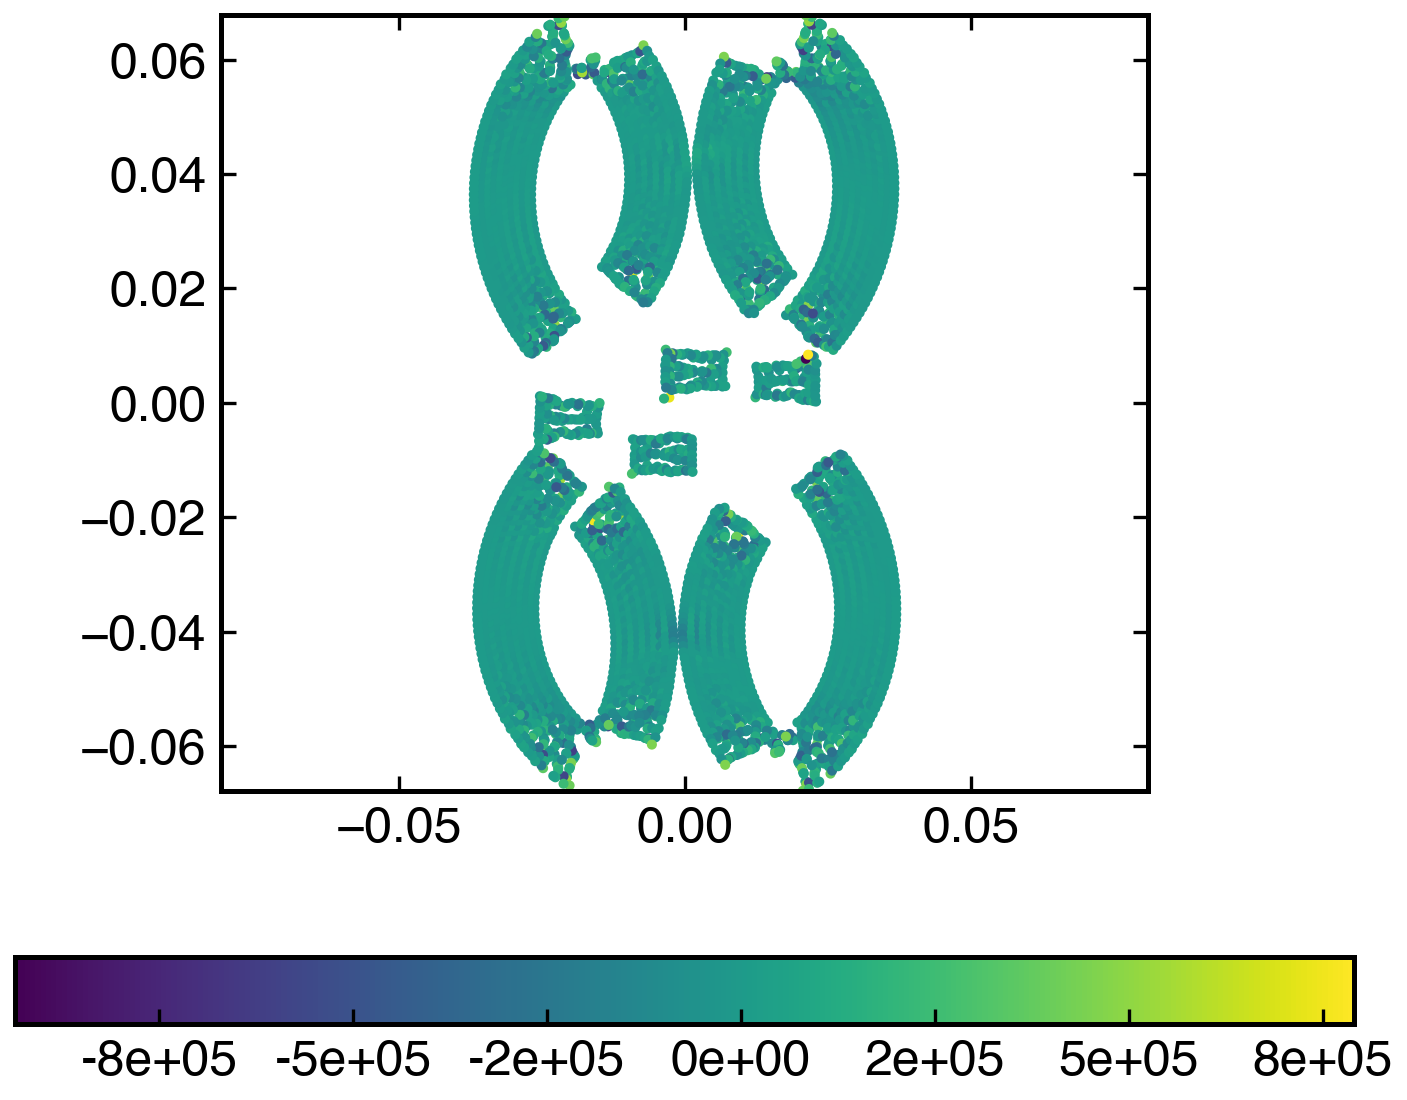
\includegraphics[width=1.0\textwidth]{figures/intro/figures/rings/time5}
% %     \subcaption{t = 1.5e-02 sec}\label{fig:rings:sun2019-nu-0.3975-5}
% %   \end{subfigure}
%   \caption{Rings with a Poisson ratio of 0.3975 colliding head on, simulated with CTVF using SPST.}
% \label{fig:rings:sun2019-nu-0.3975}
% \end{figure}
% %


\section{Summary}
We gave an overview of modeling the abrasive water jet machining. After
reviewing the possible techniques to simulate it through mesh-based schemes and
meshless methods, due to the computational limits and ease of modeling, we chose
meshless methods. Among many meshless methods, we have chosen the SPH method in
the current work, and this is due to the developed software available in the
group and work done in literature on SPH history. At the same time, DEM is used
to model the interaction between the rigid bodies. An outline of the current
thesis is set. We start with the present chapter to handle the fluid and elastic
dynamics.

In the current chapter, among all the required physics to be simulated, we have
chosen to handle the fluid and elastic dynamics. In the such process we
introduced the equations governing the fluid and structural dynamics. We
introduced the basic SPH equations and how SPH approximates functions and
derivatives. SPH is applied to solve the fluid and elastic dynamics, through
which better SPH approximations are discussed. We found that the SPH without any
corrections has several issues, like tensile instability, and inhomogeneous
particle distribution leading to poorer accuracy of the simulation. SPH has
accuracy issues, and it cannot produce 2nd order accurate results.

In the next chapter, we will propose a particle shifting technique into SPH and
move the particles with transport velocity rather than momentum velocity. And
check solve the particle homogenization problems, tensile instability. Problems
involving boundaries are handled as well.

%  We gave an overview of modeling the abrasive water jet machining. After
% reviewing the possible techniques to simulate it through mesh-based schemes and
% meshless methods, due to the computational limits and ease of modeling, we chose
% meshless methods. Among many meshless methods, we have chosen the SPH method to
% model the fluid and elastic dynamics in the current work. At the same time, DEM
% is used to model the interaction between the rigid projectiles.

%  In the current chapter, we introduce the basics of smoothed particle
% hydrodynamics. We have discussed the function, derivative and divergence
% approximations in SPH. In the next chapter, we will develop a scheme where a
% particle shifting technique into SPH and apply it to solve
